	\documentclass[10pt,oneside]{CBFT_book}
	% Algunos paquetes
	\usepackage{amssymb}
	\usepackage{amsmath}
	\usepackage{graphicx}
% 	\usepackage{libertine}
% 	\usepackage[bold-style=TeX]{unicode-math}
	\usepackage{lipsum}

	\usepackage{natbib}
	\setcitestyle{square}

	\usepackage{polyglossia}
	\setdefaultlanguage{spanish}
	



	\usepackage{CBFT.estilo} % Cargo la hoja de estilo

	% Tipografías
	% \setromanfont[Mapping=tex-text]{Linux Libertine O}
	% \setsansfont[Mapping=tex-text]{DejaVu Sans}
	% \setmonofont[Mapping=tex-text]{DejaVu Sans Mono}

	%===================================================================
	%	DOCUMENTO PROPIAMENTE DICHO
	%===================================================================

\begin{document}

% =================================================================================================
\chapter{Introducción a la mecánica cuántica relativista}
% =================================================================================================

Consideremos una partícula libre por el momento 
\[
	H = \frac{p^2}{2m} \quad E =  i\hbar \dpar{}{t} \quad \vb{p} = - i\hbar \Nabla
\]
en relatividad la primera expresión no sirve pero la segunda y la tercera sí.
\[
	P_\mu = i \hbar \partial_\mu = i \hbar \dpar{}{x^\mu}
\]
\[
	p^\mu = (E/c, \vb{p}) \qquad p_\mu = (E/c, -\vb{p}) \qquad x^\mu = (ct, \vb{x})
\]
\[
	\dpar{}{x^\mu} = \left( \frac{1}{c}\dpar{}{t} , \Nabla \right) \equiv \partial_\mu
	\qquad \dpar{}{x_\mu} = \left( \frac{1}{c}\dpar{}{t} , -\Nabla \right) \equiv \partial^\mu
\]
y Schrödinger para la partícula libre es
\be \label{schro_freepart}
	i \hbar \dpar{\psi}{t} = - \frac{\hbar^2}{2m} \nabla^2 \psi
\ee
y entonces podemos hacer la cuenta 
\[
	\psi^* \times \eqref{schro_freepart} \rightarrow  
	i \hbar \psi^*\dpar{\psi}{t} = - \frac{\hbar^2}{2m} \psi^* \nabla^2 \psi
\]
y conjugando la ecuación,
\[
	\psi \times \eqref{schro_freepart}^* \rightarrow  
	-i \hbar \psi\dpar{\psi^*}{t} = - \frac{\hbar^2}{2m} \psi \nabla^2 \psi^*
\]
y restando ambas expresiones se obtiene 
\[
	i \hbar \left( \psi^*\dpar{\psi}{t} + \psi\dpar{\psi^*}{t} \right) =
	\frac{\hbar^2}{2m} \left( \psi \nabla^2 \psi^* -\psi^* \nabla^2 \psi \right)
\]
\[
	i \hbar  \dpar{ (\psi^* \psi) }{t} + \frac{\hbar^2}{2m} 
	\Nabla \cdot \left( \psi^* \Nabla \psi - \psi \Nabla \psi^* \right) = 0
\]
la cual se puede reescribir como
\[
	\dpar{ (\psi^* \psi) }{t} +  
	\Nabla \cdot \left( \frac{\hbar}{2mi} [\psi^* \Nabla \psi - \psi \Nabla \psi^*] \right) = 0
\]
que es una analogía de la conservación de la carga en electrodinámica. Recordemos que la conservación de la carga era
$ \partial_t \rho + \nabla \cdot \vb{J} = 0$.
Tenemos entonces una especie de conservación de la probabilidad. Note que $\psi^* \psi = |\psi|^2 \geq 0$
\[
	E^2 = c^2 p^2 + m^2 c^4
\]
\[
	E = \sqrt{ c^2 p^2 + m^2 c^4 } = H \qquad \text{con} \; H\psi = E\psi
\]

Pero esto se pone muy complicado debido a la raíz

\subsection{La ecuación de Klein-Gordon}

Conserva el cuadrado para no complicar demasiado los reemplazos. Entonces 
\[
	H^2 = E^2 = c^2p^2 + m^2c^4
\]
\be \label{ec_kg}
	-\hbar \dpar[2]{\psi}{t} = - \hbar^2c^2 \Nabla^2\psi + m^2 c^4 \psi
\ee
\[
	p^\mu p_\mu = m^2c^2 \qquad -\partial_\mu\partial^\mu \psi = \frac{m^2c^2}{\hbar^2}\psi
\]
siendo el operador $\Box^2 \equiv \partial_\mu\partial^\mu$ el dalembertiano.
\[
	\left( \Box^2 + \frac{m^2c^2}{\hbar^2} \right) \psi = 0
\]
y procediendo de modo ídem al caso anterior,
\[
	\psi^* \cdot \eqref{ec_kg} = - \hbar^2 \psi^* \partial_t^2 \psi =
	- \hbar^2 c^2 \psi^* \nabla^2 \psi + m^2 c^4 \psi^*\psi
\]
\[
	\psi \cdot \eqref{ec_kg}^* = - \hbar^2 \psi \partial_t^2 \psi^* =
	- \hbar^2 c^2 \psi \nabla^2 \psi^* + m^2 c^4 \psi\psi^*
\]
y restando ambas ecuaciones tenemos
\[
	\hbar^2 \dpar{}{t}\left(  \psi^* \partial_t \psi -  \psi \partial_t \psi^* \right) =
	\hbar^2 c^2 \Nabla\cdot( \psi^* \Nabla \psi - \psi \Nabla \psi^* )
\]
\[
	\dpar{}{t}\left( \frac{i}{c^2}[ \psi^* \partial_t \psi -  \psi \partial_t \psi^* ]\right) +
	i\Nabla\cdot( \psi \Nabla \psi^* - \psi^* \Nabla \psi ) = 0
\]

El problema es que no puede asegurarse que esta $\rho \equiv i/c^2[ \psi^* \partial_t \psi -  \psi \partial_t 
\psi^* ]$ sea definida positiva, lo cual sería necesario para seguir una coherencia.
\[
	\psi = N \euler^{ i/\hbar(\pe{p}{x} - Et)}
\]
\[
	\partial_t \psi = -N \frac{iE}{\hbar} \euler^{ i/\hbar(\pe{p}{x} - Et)}
\]
\[
	\rho = \frac{i}{c^2}\left( N^*\euler^{ -i/\hbar(\pe{p}{x} - Et)}(-N)
	\frac{iE}{\hbar} \euler^{ i/\hbar(\pe{p}{x} - Et)} - 
	N \euler^{ i/\hbar(\pe{p}{x} - Et)}N^*\frac{E}{\hbar} \euler^{ i/\hbar(\pe{p}{x} - Et)}\euler^{i\pi/2}
	\right)
\]
\[
	\rho = -\frac{i}{c^2}\left( 2|N|^2 \frac{iE}{\hbar} \right) < 0 \quad \text{si} \quad E > 0
\]
para una onda plana.
Necesito considerar $E<0$ pues $E=\pm\sqrt{c^2p^2+m^2c^4}$ y la base debe ser completa.

La densidad $\rho$ es positiva si tuviese $E<0$ pero esto causa el problema de tener materia inestable, pues nunca se 
alcanza el fundamental. Acá muere en este atolladero la ecuación de Klein-Gordon.

\subsection{La ecuación de Dirac}

Dirac parte de pedir una ecuación lineal en el impulso \vb{p}
\[
	H = c \vb{\alpha} \cdot \vb{p} + \beta m c^2
\]
usando $H\psi = E\psi$ y $H^2 = E^2 = c^2p^2 + ,m^2 c^4$ y con $\beta,\vb{\alpha},\vb{p}$ operadores.
\[
	H^2 = (c \vb{\alpha} \cdot \vb{p} + \beta m c^2)(c \vb{\alpha} \cdot \vb{p} + \beta m c^2)
\]
\[
	H^2 = c^2 \alpha_i p_i \alpha_\ell p_\ell + c^3 \alpha_i p_i \beta m +
	\beta m c^3 \alpha_i p_i + \beta^2 m^2 c^4
\]
\[
	H^2 = c^2 \alpha_i \alpha_\ell p_i  p_\ell + c^3 m p_i \underbrace{( \alpha_i \beta + \beta \alpha_i )}_{=0}
	+ \beta^2 m^2 c^4
\]
\[
	H^2 = 
	c^2 \underbrace{\left( \frac{\alpha_i \alpha_\ell + \alpha_\ell\alpha_i}{2} \right)}_{\delta_{i\ell}}
	p_i p_\ell + m^2 c^4 \underbrace{\beta^2 }_{ = 1 }
\]
\[
	\alpha_i \alpha_\ell + \alpha_\ell\alpha_i = 2 \delta_{i\ell} \qquad 
	\alpha_i \beta + \beta \alpha_i= 0 \qquad
	\beta^2 = 1
\]
Como se ve, estos no pueden ser simples escalares. Dirac pide 
\begin{itemize}
 \item $\vb{\alpha},\beta$ hermíticos
 \item $\beta^2=1 \; \alpha^2=1$ autovalores $\pm 1$
 \item traza nula
 \[
	\alpha_i \beta = -\beta \alpha_i  \quad \rightarrow  \quad 
	\beta \alpha_i \beta = -\beta^2 \alpha_i = -\alpha_i
 \]
 \[
	Tr(\alpha_i) = -Tr(\beta \alpha_i \beta) = -Tr(\beta\beta\alpha_i)
 \]
 \item dimensión par 
 \[
	\vb{\alpha} = \begin{pmatrix} 0 & \vec{\sigma} \\ \vec{\sigma} & 0 \\ \end{pmatrix} \qquad 
	\beta = \begin{pmatrix} \mathbb{1} & 0 \\ 0 & -\mathbb{1} \\ \end{pmatrix}
 \]
 donde cada elemento de la matriz es de $2\times2$.
\end{itemize}

Entonces
\[
	H \vec{\psi} = i \hbar \dpar{\vec{\psi}}{t}, \qquad H \in 4\times 4, \vec{\psi} \in 4\times 1, \qquad
	\vec{\psi} = \begin{pmatrix} \psi_1 \\ \psi_2 \\ \psi_3 \\ \psi_4 \end{pmatrix}
\]
\be \label{ec_dirac}
	i \hbar \dpar{\psi}{t} = -i \hbar c \sum_k \alpha_k \dpar{\psi}{x_k} + m c^2 \beta \psi
\ee
\[
	-i \hbar \dpar{\psi^\dagger}{t} = i \hbar c \sum_k \dpar{\psi^\dagger}{x_k}\alpha_k + m c^2\psi\alpha_k\beta
\]
\[
	\psi^\dagger\cdot\eqref{ec_dirac} - \eqref{ec_dirac}^\dagger\cdot \psi \rightarrow 
	i\hbar \dpar{}{t}(\psi^\dagger psi) = -i\hbar c \sum_k \dpar{}{x_k}(\psi^\dagger \alpha_k \psi)
\]
\[
	\dpar{}{t}(\psi^\dagger psi) + c \sum_k \dpar{}{x_k}(\psi^\dagger \alpha_k \psi) = 0
\]
Y si $\rho \equiv \psi^\dagger\psi$ ahora tenemos una densidad de proababilidad como requiere la naturaleza.

\subsection{Ejemplo: partícula libre quieta}

Sea una partícula libre en reposo,
\[
	\vb{p} = 0 \qquad H=\beta m c^2
\]
\[
	i \hbar \dpar{\psi}{t} = \beta m c^2 \psi
\]
\[
	i \hbar \dpar{}{t} \begin{pmatrix} \psi_1 \\ \psi_2 \\ \psi_3 \\ \psi_4  \end{pmatrix} =
	\begin{pmatrix} mc^2 & 0 & 0 & 0 \\ 0 & mc^2 & 0 & 0 \\ 0 & 0 & -mc^2 & 0 \\ 0 & 0 & 0 & -mc^2 \end{pmatrix}
	\begin{pmatrix} \psi_1 \\ \psi_2 \\ \psi_3 \\ \psi_4  \end{pmatrix}
\]
Tenemos cuatro ecuaciones, dos con energía positiva y dos con energía negativa
\[
	i \hbar \dpar{\psi_i}{t} = mc^2 \psi_i \qquad i \hbar \dpar{\psi_i}{t} = -mc^2 \psi_i
\]
\[
	\psi_1 = \euler^{-imc^2t/\hbar}\begin{pmatrix} 1 \\ 0 \\ 0 \\ 0  \end{pmatrix} \qquad 
	\psi_3 = \euler^{imc^2t/\hbar}\begin{pmatrix} 0 \\ 0 \\ 1 \\ 0  \end{pmatrix}
\]
Como aún tenemos degeneración de orden dos, necesitaremos un operadore que conmute con el $H$
\[
	\vec{\Sigma} = \begin{pmatrix} \vec{\sigma} & 0 \\ 0 & \vec{\sigma} \\ \end{pmatrix} \qquad 
	[H,\vec{\Sigma}] = 0
\]
\[
	\Sigma_3 =  \begin{pmatrix} \sigma_3 & 0 \\ 0 & \sigma_3 \\ \end{pmatrix} = 
	\begin{pmatrix} 1 & 0 & 0 & 0 \\ 0 & -1 & 0 & 0 \\ 0 & 0 & 1 & 0 \\ 0 & 0 & 0 & -1 \end{pmatrix}
\]
\begin{align*}
	\psi_1, E=mc^2, \Sigma_3=1 \qquad  &\psi_2, E=mc^2, \Sigma_3=-1 \\
	\psi_3, -E=mc^2, \Sigma_3=1 \qquad  &\psi_4, -E=mc^2, \Sigma_3=-1
\end{align*}
Podemos identificar 
\[
	\vec{S} = \frac{\hbar}{2} \vec{\Sigma}
\]
\[
	\text{si} \; p \neq 0  \Rightarrow [H, \vb{\Sigma}] = 2ic \vb{\alpha} \times \vb{p}
\]

\subsection{Energías negativas}

Como $E = \pm  \sqrt{ c^2 p^2 + m^2 c^4 } $ hay $E<0$ y además un {\it gap} de ancho $2mc^2$ entre ellas.
Las $E<0$ harían que la materia jamás alcance un estado fundamental y por ende jamás se estabilice.
Dirac piensa que los estados de $E<0$ están todos llenos. No decaen más electrones allí dentro. Es el mar de 
Dirac. Iluminando ese vacío se lo puede excitar.

\begin{figure}[htb]
	\begin{center}
	\includegraphics[width=0.6\textwidth]{images/teo2_13.pdf}
	\end{center}
	\caption{}
\end{figure} 

Podemos hacer saltar a la zona positiva una carga $(-e)$ dejando un huevo positivo (equivalente a una carga 
$+e$). Es una creación e pares $\gamma \to e^-e^+$, sin embargo el proceso inverso $ e^-e^+ \to \gamma$ de 
aniquilación de pares ocurre prontamente.
Se observó experimentalmente.

\begin{figure}[htb]
	\begin{center}
	\includegraphics[width=0.6\textwidth]{images/teo2_14.pdf}
	\end{center}
	\caption{}
\end{figure} 

Fotos extra para el asunto de las energías negativas a continuación:

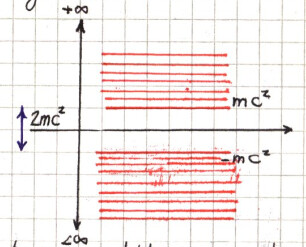
\includegraphics[width=0.6\textwidth]{images/fig_ft2_energias_negativas_1.jpg}

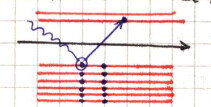
\includegraphics[width=0.6\textwidth]{images/fig_ft2_energias_negativas_2.jpg}

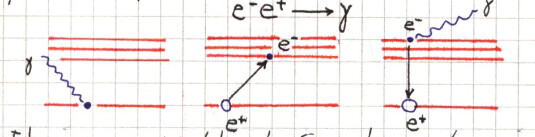
\includegraphics[width=0.6\textwidth]{images/fig_ft2_energias_negativas_3.jpg}


% \bibliographystyle{CBFT-apa-good}	% (uses file "apa-good.bst")
% \bibliography{CBFT.Referencias} % La base de datos bibliográfica

\end{document}
